 \documentclass{report}
\usepackage{setspace}
\doublespacing
\usepackage[utf8]{inputenc}
\usepackage{graphicx}
\usepackage{amsmath}
\usepackage{indentfirst}
\usepackage[labelfont=bf]{caption}
\usepackage{array, boldline, makecell, booktabs}
\newcommand\btrule[1]{\specialrule{#1}{0pt}{0pt}}

\title{Polyphase Filter Banks: A Physicist's Attempt}
\author{Matthew Cooper}
\date{Sometime in May, 2019}
\begin{document}
\maketitle

\tableofcontents{}

\newpage
\chapter{Introduction}

In the modern era, the speed of digital processing components has made it such that the gap between digital and analog is becoming ever smaller, allowing us the advantages that come with conversion of analog signals to digital signals.  These advantages are numerous, but, as with anything, there is an equivalent exchange, and there are tradeoffs in using digital signals which, if not taken into account, can turn a scientific data product into something completely unusable.

In my researching of this subject, it became clear early on that my understanding of the fundamentals that go into digital signal processing (DSP hereafter) were not up to par, which resulted in several hours of researching different aspects of DSP in order to complete the mental picture I needed.  It is my goal in the pages of this report to recreate, as best I can, this journey, making pitstops at different ideas that helped shape my current, albeit incomplete understanding.  

The first reference I was able to find for polyphase filter bank implementation was a paper from 1973 (Schafer and Rabiner, 1973).  In this paper, however, the term polyphase had not been coined yet.  Its original implementation was to increase resolution of frequency channels for speech analysis and synthesis.  Not suprising, this came out of Bell Labs.  We'll discuss this paper in greater detail when we come to the theory side of things.

Although it started as a method of reconstructing speech output, the applications of polyphase filter banks has found use in almost all areas where channelization is required, such as cell phone signal downconversion and up conversion (Harris, 2003), as well as being considered for implementation in the Extended Owens Valley Solar Array(CITE).  

In this report, we will review some basics of analog-to-digital conversion, methods which have been created to navigate the restrictions that such conversions place on the type of data which can be sampled, and then proceed with how polyphase filter banks are utilized in the optimization of such a process.  

\chapter{Fundamentals of Digital Signals}
\section{Analog Vs. Digital}

The filtering and manipulation of analog signals has been widely used for decades.  Why, then, is there the push for analog-to-digital conversion?  For systems where the average power of a signal is the only necessity, staying in the analog domain is perfectly acceptable.  The issue arises when a system also needs to accurately measure and record phase information.  In analog systems, the gain to phase balance of a signal cannot be maintained to better than $1\%$ over a range of temperatures (Harris, 2003).  

\begin{figure}[ht]
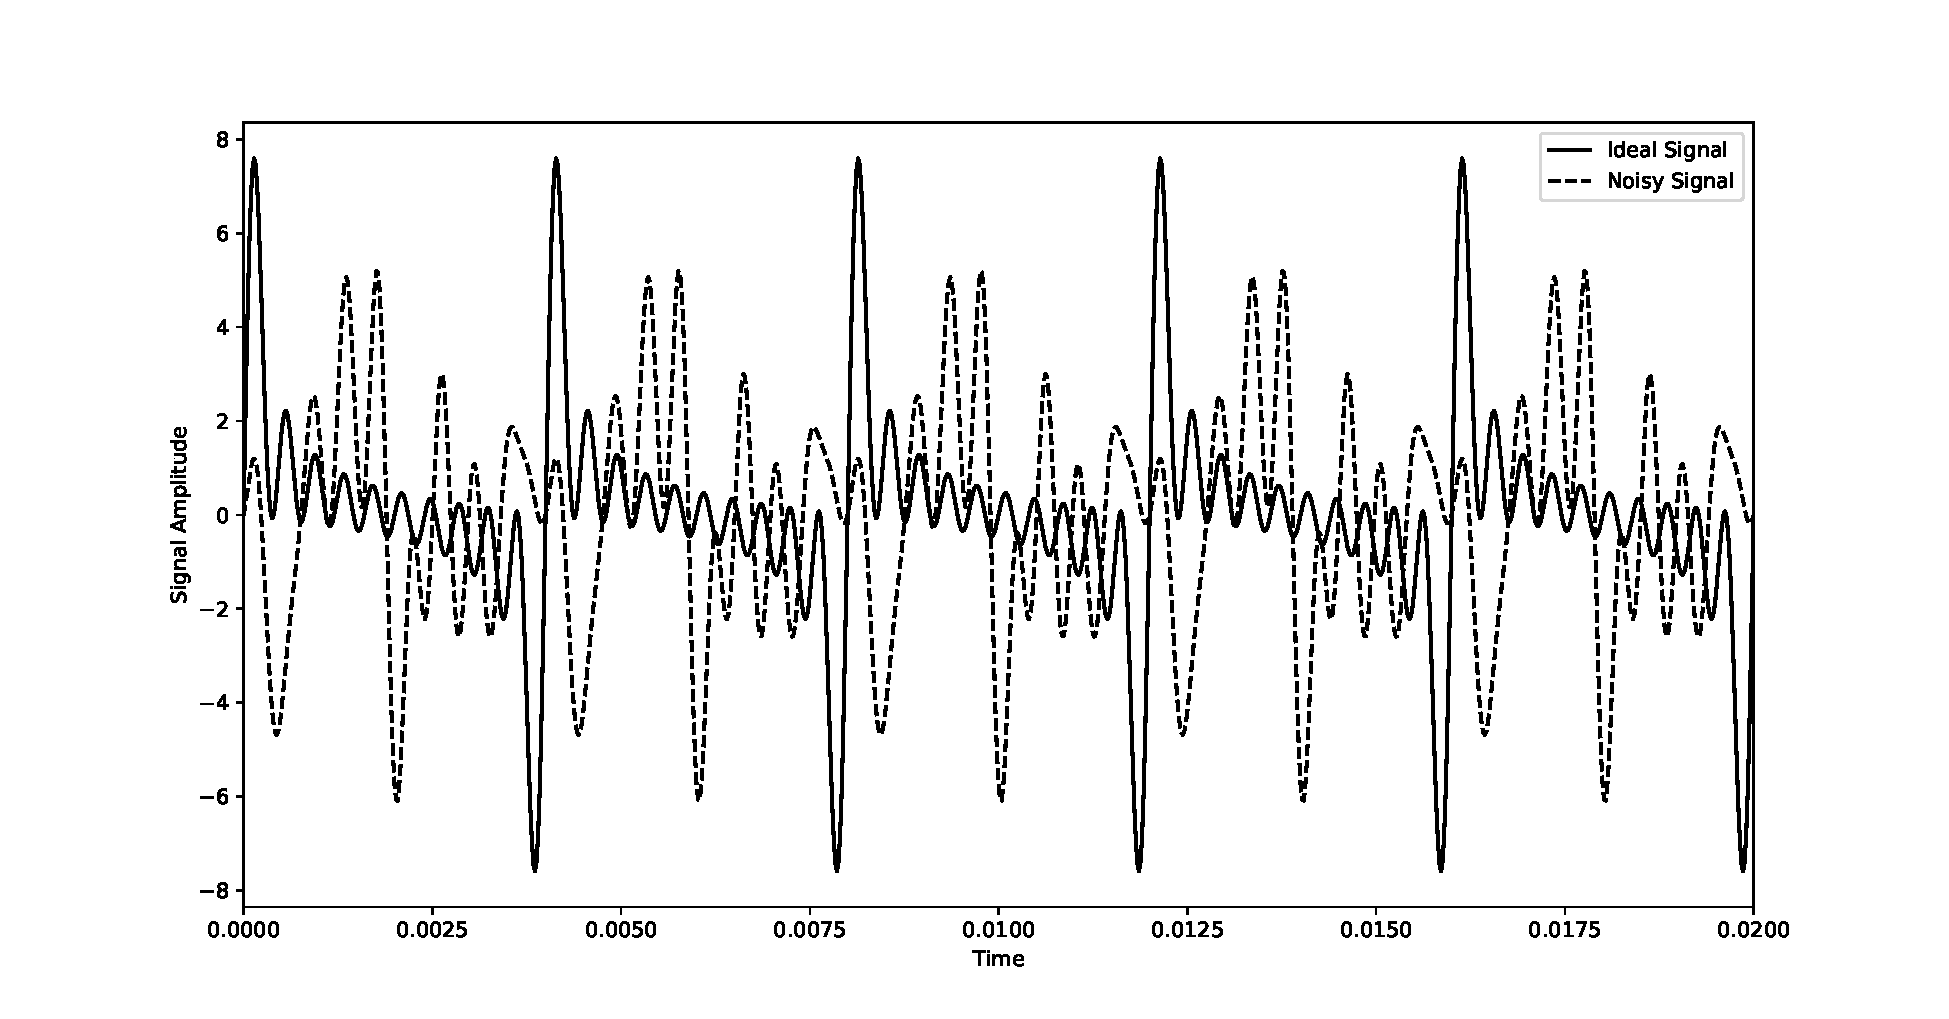
\includegraphics[scale=.45]{Figure_4.pdf}
\caption{Plotted above is an ideal signal which has had uncertainty introduced in its phase and amplitude profile.}
\end{figure}

Figure 1.1 gives an example of the error which can be introduced by such errors.  This is particularily crippling for a multi-antennae radio array, which relies on phase-locking between antennae in order to steer the beam.  Since no two antennae's analog components can match identically, leaving the signal in the analog domain can produce spurious phase shifts, which are functions of many variables which cannot be accounted for simply, if at all.  This is where analog-to-digital conversion is helpful, since the phase information stored in a digital signal is not subject to environmental effects.  

\section{Analog Signal Sampling}

In analog-to-digital conversion, there are two relations which must be considered: the Nyquist Sampling Theorem, and the Frequency Resolution Relation.  These combined determine the sampling rate which must be attained in order to recover a maximum frequency, as well as how much resolution there will be between frequencies.  The Nyquist Theorem (Landau, 1967) states that
\begin{equation}
f_{crit} = \frac{f_{sample}}{2}
\end{equation}

where $f_{crit}$ is the maximum frequency which can have power 'definitively' attributed to it (i.e. has no alias), and $f_{sample}$ is the sampling frequency.  This relation is troubling for radio transmissions.  Consider a 10 GHz signal.  In order to recover this signal, it must be sampled at 20 billion samples per second.  At 64 bit resolution, this equates to around 160 Gigabytes of data.  Currently, FPGA's on the market sit in the MHz processing speed range, although ADC converters currently exist which can handle giga-samples per second.

The second relation, the Frequency Resolution Relation, gives a size requirement for the hardware register which must be fed to the FFT in order to maintain a specific resolution between frequencies.
\begin{equation}
f_{res} = \frac{f_{sample}}{N}
\end{equation}

where $f_{res}$ is the resolvability.  So, for higher sample rates, the register size must also increase to maintain frequency resolvability.  Clearly, a register which is of the order of 160 Gigabytes is something science fiction would hesitate to create, so how is this issue circumvented? The obvious answer is to sample less, but therein lies the problem, since in the process we lose information either by loss of resolution or by ambiguity in frequency aliasing.  The method which was created to circumvent this problem was the concept of downconversion.

\section{Downconversion}

Downconversion (heterodyning) was originally worked on by Nikola Telsa and Reginald Fessenden (Espenschied 1959).  Fessenden patented the heterodyne principle in 1902, and that same year founded the National Electrical Signaling Company (NESCO).  John Vincent Lawless Hogan, who went to work for Fessenden in 1910, showed how the concept had greatly improved the sensitivity of radio receivers (Godara, 1999).  The introduction of this concept revolutionized electromagnetic signaling, and it is no stretch to say that without it, the subject of this paper, as well as many other DSP related ideas, would never have existed.

What is heterodying? Heterodyning is the process by which a signal is mixed with a higher frequency signal in order to mirror the signal to a lower frequency band.  This can be easily shown mathematically.  Consider a monochromatic input signal, $x_{in}$, and a local signal, $x_{lo}$.  Then,
\begin{align}
x_{in}*x_{lo}& = sin(f_{in}t)sin(f_{lo}*t)\\
             & = \frac{1}{2}[cos((f_{lo}-f_{in})*t) - cos((f_{lo}+f_{in})*t]
\end{align}

Here, we see that there are two mirrors of the input signal; one which is at higher frequencies, and one which is at lower frequencies, with an example shown in Figure 1.  
\begin{figure}[ht]
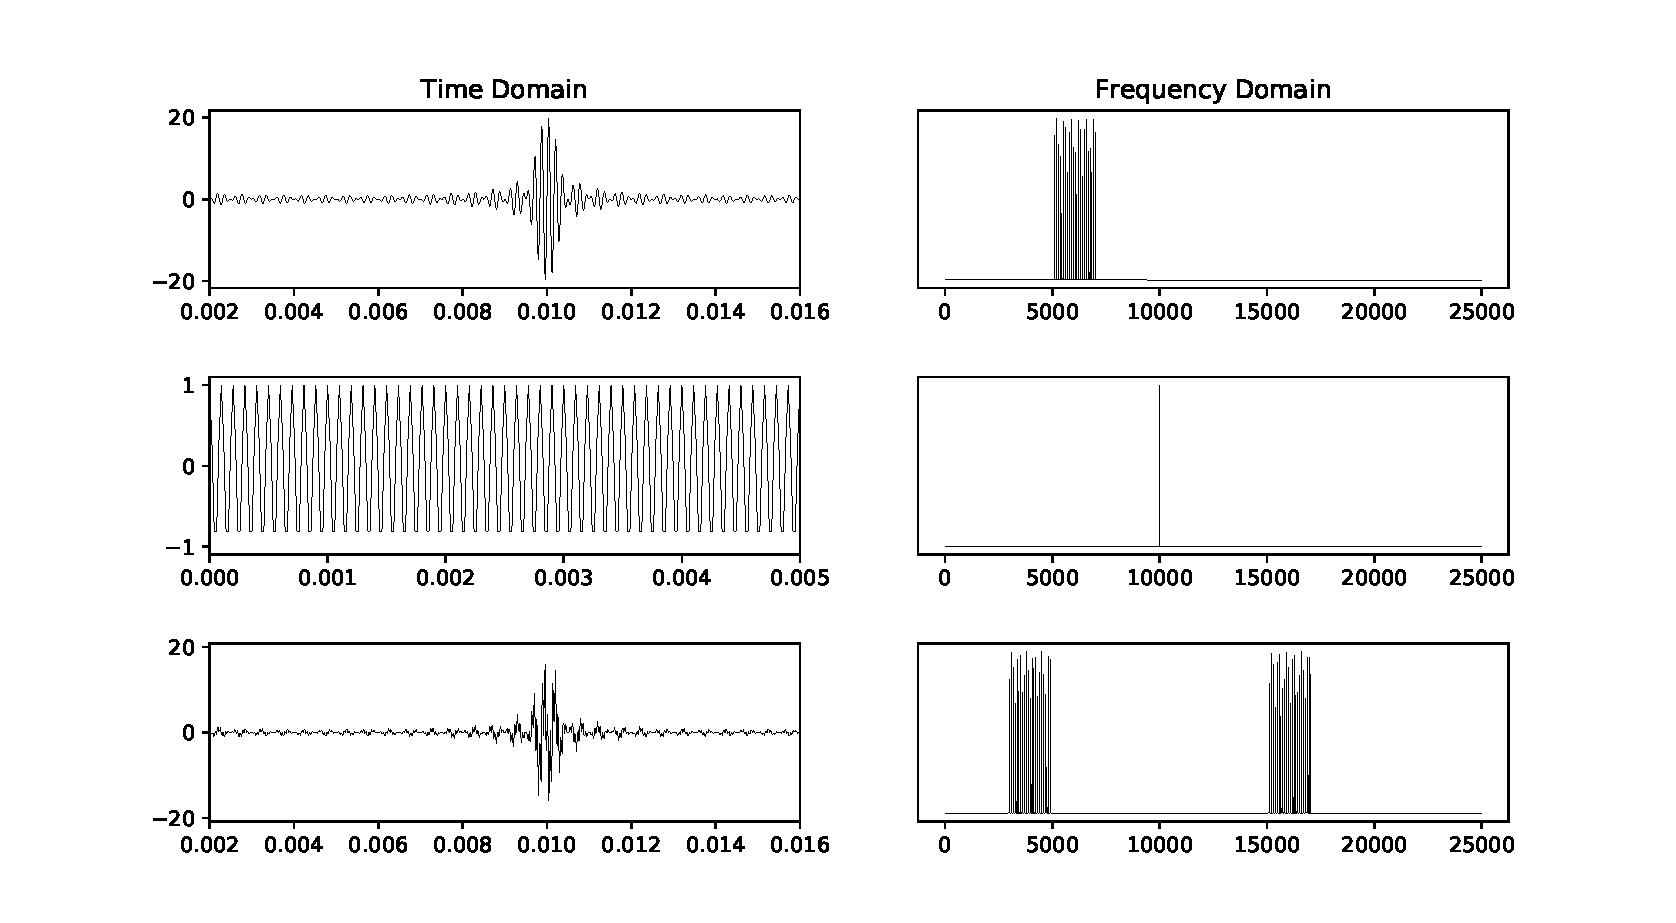
\includegraphics[scale=.45]{Figure_1.pdf}
\caption{(top) Signal $x_{in}$ in the time and frequency domain (middle) Signal $x_{lo}$ in time and frequency domain (bottom) Signal $x_{in}x_{lo}$ in the time and frequency domain}
\end{figure}

The part we are interested in is, of course, the lower frequencies, since we don't have to sample these as often.  Therefore, the higher frequency components must be removed.  We remove these signal contributions by the process of filtering.

\section{Digital Signal Filters}

Digital signal filters are arguably one of the biggest fields within the realm of electrical engineering, and for good reason.  This process allows one to attenuate certain frequency bands, while leaving others (relatively) unaffected. 

\begin{figure}[ht]
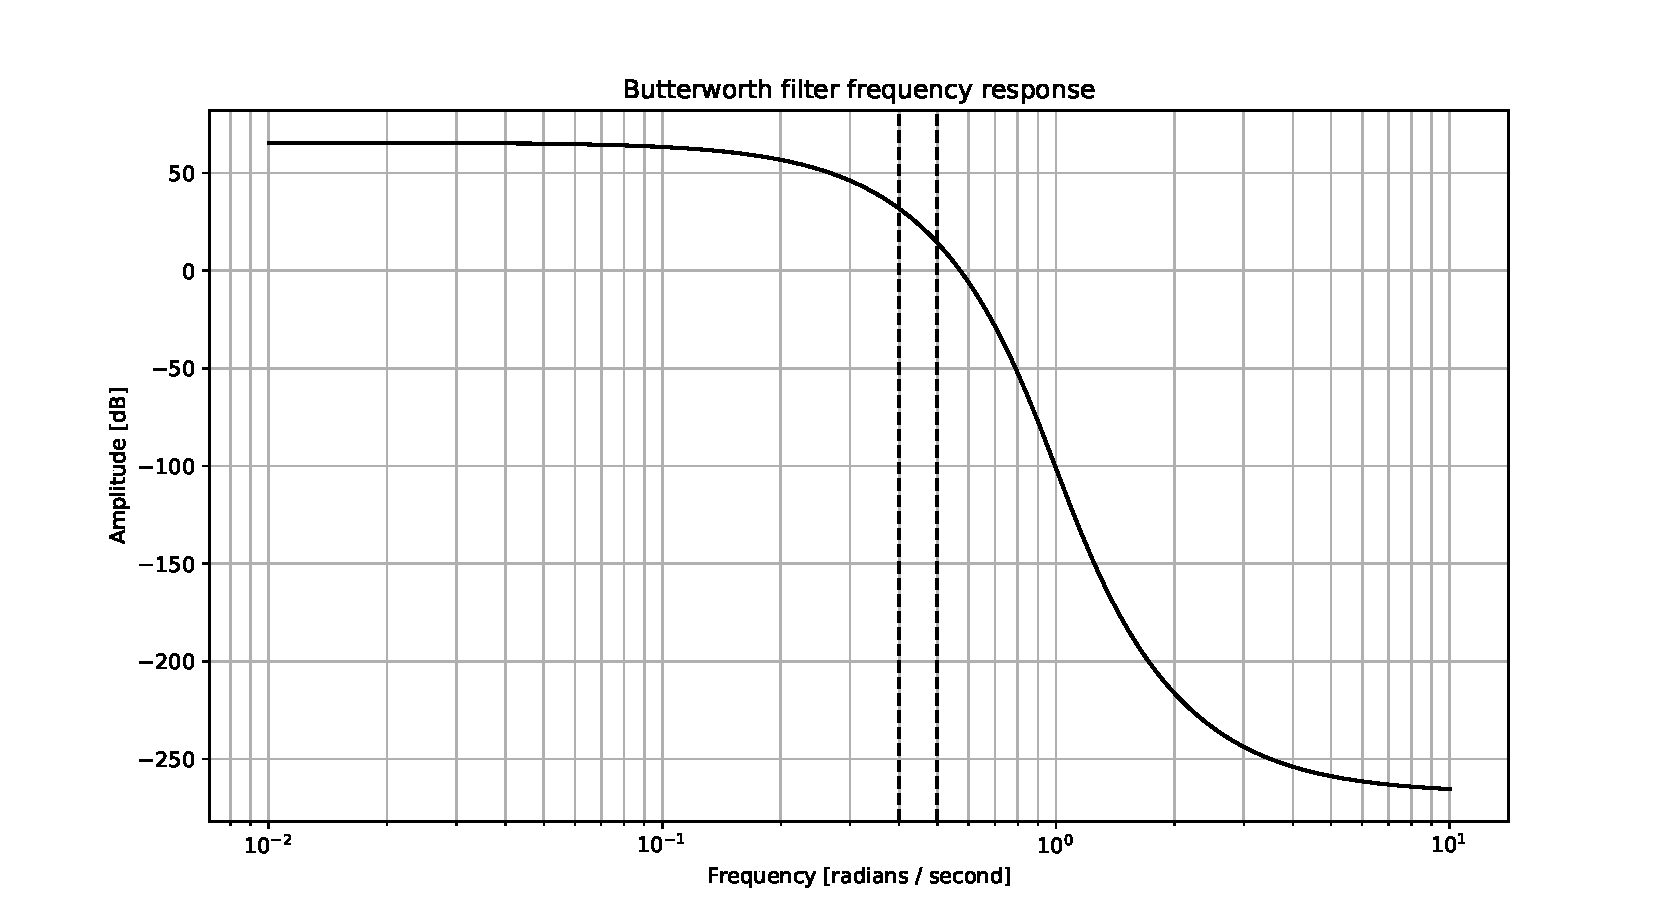
\includegraphics[scale=.45]{Figure_2.pdf}
\caption{Plotted above is the frequency responses for a Butterworth filter of low-pass type.  The y-axis indicated the attenuation (in dB) of the different frequency components.  The first dashed line indicated the end of the pass-band, and the second is the beginning of the stop band.}
\end{figure} 

Figure 2.3 shows a typical frequency response profile for a filter transfer function.  As can be seen, all frequencies are affected, but the stopband frequences are attenuated much more heavily than in the passband.  Other filter types, such as Chebyshev, Bessel, and Elliptic, have other features which would appear in such a plot.  The Butterworth filter has no rippling in the attenuation of its passband, whereas an Elliptic or Bessel filter would.  Thus, different filters are chosen for different applications.  Specific bandstop filters have been created for radio astronomy in particular, such as the cryogenic S-band filter, which is a hardware bandstop filter which mimics a Chebyshev/Elliptic bandpass filter (Srikanta, 2012).  This filter differs from digital filters in that it cannot have its bandwidth adjusted.  A digital filter can be altered simply by changing the coefficient register in the FPGA.

Signal filters are commonly derived in the Laplace domain, due to the simplicity of the mathematics.  The task is then to convert it to the Z-domain, via transforms such as a bilinear transform.  One then takes the impulse response of a given filter, which for an FIR filter gives the coefficients with which to convolve the input signal, via.
\begin{equation}
y[n] = \sum^{N-1}_{k=0}x[k]h[n-k]
\end{equation}
Example time-domain coefficients for the Butterworth filter above are given in Figure 2.2. The results of such a convolution can be observed in Figure 2.5, where we have taken the down-converted signal from above and implemented a bandpass Butterworth filter.  This signal can now be decimated (down-sampled) without any loss of information.
 
\begin{figure}[!ht]
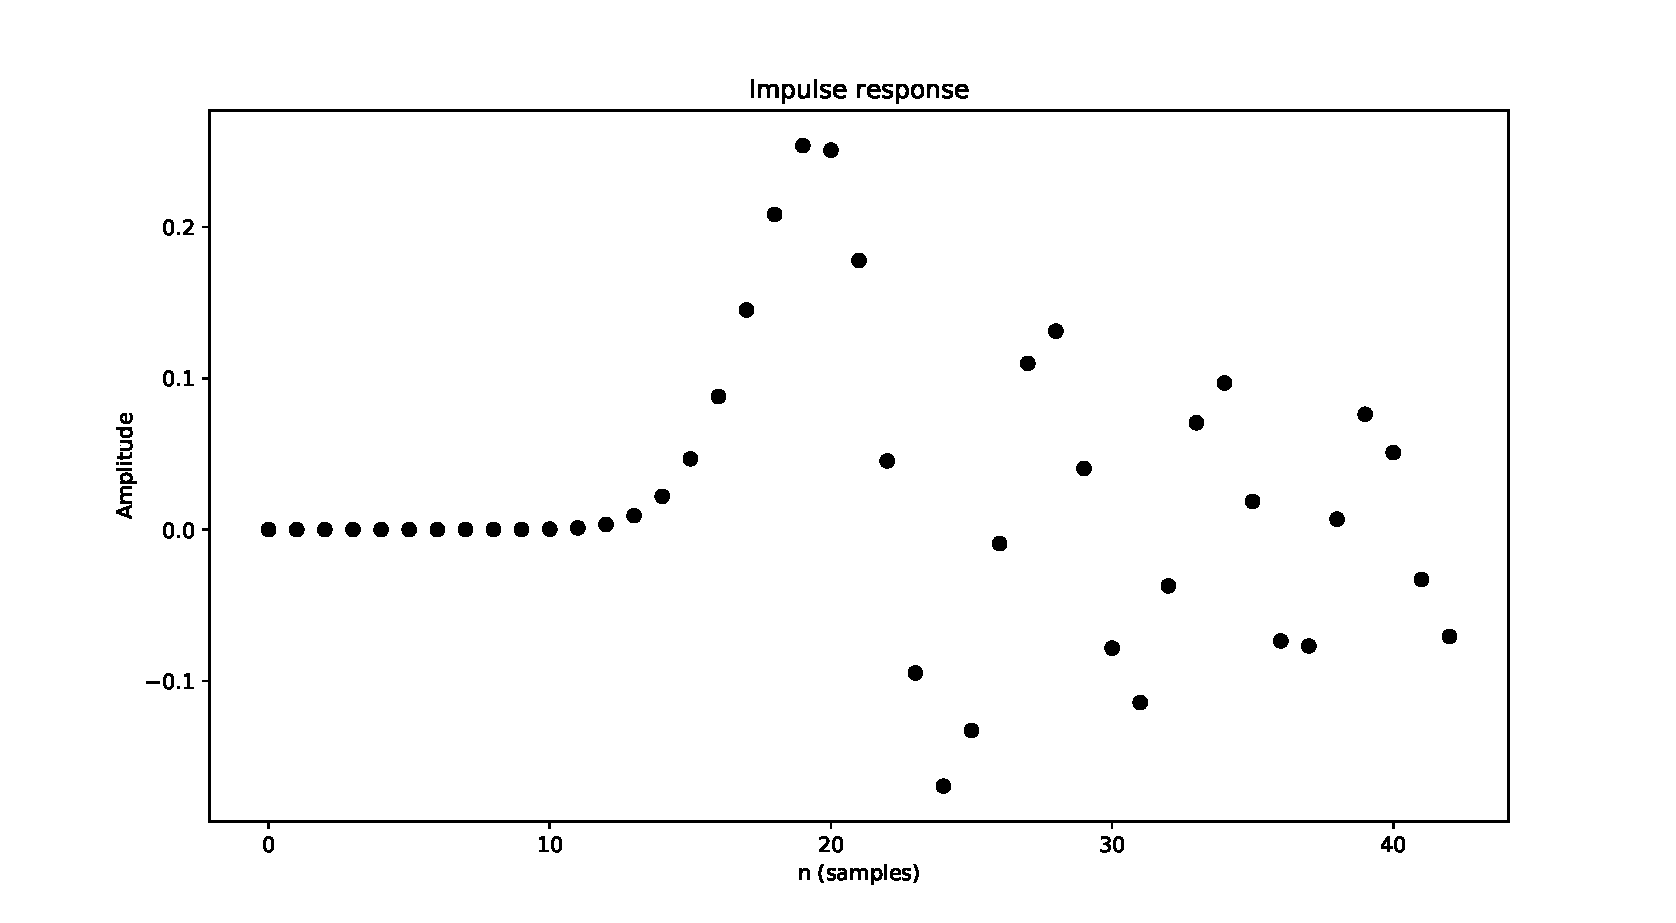
\includegraphics[scale=.4]{Figure_3.pdf}
\caption{Plotted above is the impulse response, h[n], for a Butterworth filter of low-pass type.  The y-axis indicated the coefficient value.}
\end{figure} 
\begin{figure}[!ht]
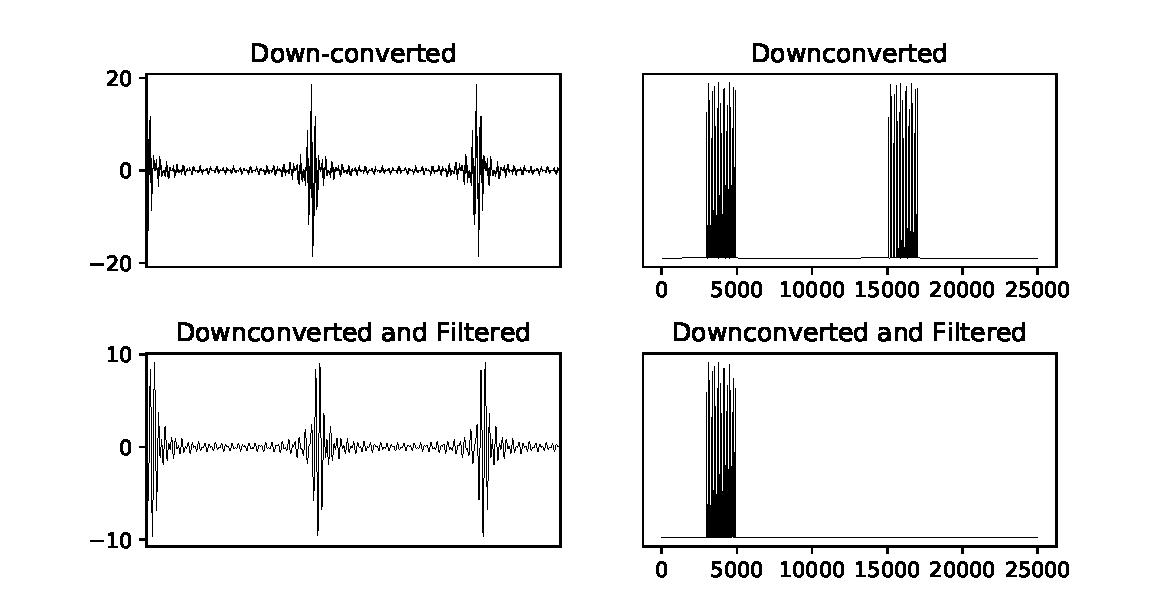
\includegraphics[scale=.6]{Figure_5.pdf}
\caption{(top) Downconverted signal and its Fourier Transform.  (bottom) Downconverted and filtered signal and its Fourier Transform.}
\end{figure} 



\section{Summary}
In this section, we have gone through the steps a signal takes after being measured by a front end system and converted to a digital signal.  This process involves sampling as a given rate, downconverting to a lower/higher frequency band, filtering to remove the high frequency component, then decimating the low frequency result.  As one can imagine, this process can be very hardware expensive.  Are there ways to make this process more efficient? It happens to be the topic of this paper.


\chapter{Polyphase Implementation}

Up to this point, we have discussed the individual components that make up digital signal processing.  What, then, is a polyphase filter bank?  A polyphase filter bank (PFB) is a method of deconstructing the input signal and filter in order to more efficiently carry out the convolution-decimation process which was outlined above.  In a direct implementation, as will be shown below, several of the multipications and additions are unnecessary, as this data will be discarded during the decimation process.  The PFB allows one to avoid these extra calculations, thus limiting the amount of hardware needed, which is especially important when utilizing finite-space FPGA boards.
\section{Theory}
This section will rely heavily on (Schafer and Rabiner, 1973).  They begin by defining a series of bandpass filters as 
\begin{equation}
h_k(n) = h(n)cos(w_kn)
\end{equation}
where $\omega_k=\triangle\omega * k$, where $\triangle\omega$ is the distance between center frequencies of adjacent channels and k is an integer value.  The filter for the entire band is then
\begin{equation}
\widetilde{h}(n) = \sum_k^M h_k
\end{equation}

which, when substituted in, yields
\begin{align}
\widetilde{h}(n) = h(n)\sum_k^M cos(w_kN)
& = h(n)d(n)
\end{align}

Schafer and Rabiner showed that if $\triangle \omega = \frac{2\pi}{NT}$, and $M = \frac{N-1}{2}$, where M is the number of channels, then 
\begin{equation}
d(n) = \frac{sin(\pi n)}{sin(\frac{\pi n}{N})}
\end{equation}

They go on to show that if one were to introduce a delay in d(n), they can remove phase echos which occur during the filtering process.  The relation to the implementation below is reasonable.  We split the filter and signal into subfilters and subsignals, as they have done with the channels.  We then time delay the filters relative to one another, as they show here, and as (Harris, 2003) shows.  In (Harris, 2003), this time delay is given as an unit delay, however.
\section{2-tap Example}
This section provides a mathematical walkthrough of a simple 2-tap polyphase implementation.  It suffices to exhibit the time delay which the second filter must have in order to recover the same output as the direction convolution-decimation. 
In a direct computation of the convolution of a signal/filter pair, as shown in Figure 3.1, where the signal is $x[n] = \{x_0, x_1, x_2, x_3, x_4, x_5\}$, and the filter is $h[n] = \{h_0, h_1, h_2, h_3\}$, where the lengths are L=6 and M=4, respectively,
\bigskip
\begin{figure}[ht]
\begin{center}
  \begin{tabular}{ l|c|c|c|c|c|c|c|r }
    \hline
    $h_0 x_0$ & $h_0 x_1$ & $h_0 x_2$ & $h_0 x_3$ & $h_0 x_4$ & $h_0 x_5$ & 0 & 0 & 0\\ \hline
    0 & $h_1 x_0$ & $h_1 x_1$ & $h_1 x_2$ & $h_1 x_3$ & $h_1 x_4$ & $h_1 x_5$ & 0 & 0\\ \hline
    0 & 0 &$h_2 x_0$ & $h_2 x_1$ & $h_2 x_2$ & $h_2 x_3$ & $h_2 x_4$ & $h_2 x_5$ & 0\\ \hline
    0 & 0 & 0 &$h_3 x_0$ & $h_3 x_1$ & $h_3 x_2$ & $h_3 x_3$ & $h_3 x_4$ & $h_3 x_5$ \\\Xhline{1pt}
    $y_0$ & $y_1$ & $y_2$ & $y_3$ & $y_4$ & $y_5$ & $y_6$ & $y_7$ & $y_8$\\ \hline
  \end{tabular}
\end{center}
\caption{The above table represents the computations necessary to implement a direction convolution.  Each column in the table is summed to create the $y_i$ coefficients at the bottom.}
\end{figure}


We can easily see that there are 24 multiplications (L*M), and 27 additions (M-1)*(L+M-1).  Now, if we change our sample rate, as shown in Figure 3.2, 

\begin{figure}[ht]
\begin{center}
  \begin{tabular}{ l|l }
    \hline
    Before Decimation & After Decimation\\ \Xhline{1pt}
	$y_0 = h_0 x_0$ & $y_0 = h_0 x_0$\\ \hline
	$y_1 = h_0 x_1 + h_0 x_1$ & 0\\ \hline 
	$y_2 = h_0 x_2 + h_1 x_1 + h_2 x_0$ & $y_2 = h_0 x_2 + h_1 x_1 + h_2 x_0$\\ \hline 
	$y_3 = h_0 x_3 + h_1 x_2+ h_2 x_2 + h_3 x_1$ & 0 \\ \hline 
	$y_4 = h_0 x_4 + h_1 x_3+ h_2 x_2 + h_3 x_1$ & $y_4 = h_0 x_4 + h_1 x_3+ h_2 x_2 +     	h_3 x_1$\\ \hline
	$y_5 = h_0 x_5 + h_1 x_4 + h_2 x_3 + h_3 x_2$ & 0\\ \hline
	$y_6 = h_1 x_5 + h_2 x_4 + h_3 x_3$ & $y_6 = h_1 x_5 + h_2 x_4 + h_3 x_3$\\ \hline
	$y_7 = h_2 x_5 + h_2 x_4$ & 0\\ \hline
	$y_8 = h_3 x_5$ & $y_8 = h_3 x_5$\\ \hline
  \end{tabular}
\end{center}
\caption{In the above left column are the coefficients produced by the direct convolution, and in the above right the coefficients remaining after a 2-tap decimation (every other sample).}
\end{figure}

we see that large fraction of the multiplications and additions that were carried out have now been through away.  Now we show how a polyphase implementation avoids these unnecessary computations.  First, we split the filter into N-tap subfilters, in this case N=2, which gives $h[n]^+ = \{h_0, h_2\}$ and $h[n]^- = \{h_1, h_3\}$.  We then convolve each of these with a sub-band of the input signal, $x[n]$, which are $x[n]^+ = \{x_0, x_2, x_4\}$ and $x[n]^- = \{x_1, x_3, x_5\}$, respectively.  These convolutions are shown in Figure 3.3 and 3.4.

\smallskip
\begin{figure}[ht]
\begin{center}
  \begin{tabular}{ c|c|c|c }
	\hline
	$h_0 x_0$ & $h_0 x_2$ &$h_0 x_4$&0\\ \hline
	0 & $h_2 x_0$ & $h_2 x_2$ &$h_2 x_4$\\ \Xhline{1pt}
	$y^+_0$ & $y^+_1$ & $y^+_2$ & $y^+_3$\\ \hline
  \end{tabular}
\end{center}
\caption{This table represents the convolution of $h[n]^+$ and $x[n]^+$.}
\end{figure}

If we count up the number of multiplications from this, we see that now there are only 12 which must be carried out.  We have thus reduced the number of multiplications by half, which for a 2-tap decimation seems reasonable.  However, we have also lowered the number of summations, from 27 to 13.  
\smallskip
\begin{figure}[ht]
\begin{center}
  \begin{tabular}{ c|c|c|c }
	\hline
	$h_1 x_1$ & $h_1 x_3$ &$h_1 x_5$&0\\ \hline
	0 & $h_3 x_1$ & $h_3 x_3$ &$h_3 x_5$\\ \Xhline{1pt}
	$y^-_0$ & $y^-_1$ & $y^-_2$ & $y^-_3$\\ \hline
  \end{tabular}
\end{center}
\caption{This table represents the convolution of $h[n]^-$ and $x[n]^-$.}
\end{figure}

Now, we combine the results of these two separate convolutions, but as we saw in the theory, we take the second output to be delayed by a timestep, which effects a spectral folding of sorts, but with the added benefit of the stopband phase offsets destructively cancelling one another.
\smallskip
\begin{figure}[!ht]
\begin{center}
  \begin{tabular}{|c|c|l}
    \hline
    First Filter & Second Filter &Convolution and Decimation\\ \Xhline{1pt}
	$y^+_0=h_0x_0$ & $y^-_{-1} = 0$ & $y^+_0 + y^-_{-1}= h_0 x_0 = \mathbf{y_0}$\\ \hline
	$y^+_1=h_0x_2+h_2x_0$ & $y^-_0=h_1x_1$ & $y^+_1 + y^-_0 = h_0 x_2 + h_1 x_1 + h_2 x_0 = \mathbf{y_2}$\\ \hline 
	$y^+_2=h_0x_4+h_2x_2$ & $y^-_1=h_1x_3+h_3x_1$ & $y^+_2 + y^-_1 = h_0 x_4 + h_1 x_3+h_2 x_2 + h_3 x_1 = \mathbf{y_4}$\\\hline
	$y^+_3=h_2x_4$ & $y^-_2=h_1x_5+h_3x_3$ & $y^+_3 + y^-_2 = h_1 x_5 + h_2 x_4 + h_3 x_3 = \mathbf{y_6}$\\ \hline
	$y^+_4=0$ & $y^-_3=h_3 x_5$ & $y^+_4 + y^-_3 = h_3 x_5 = \mathbf{y_8}$\\ \hline
  \end{tabular}
\end{center}
\caption{The table above shows how the coefficients of the separate convolutions are summed.}
\end{figure}

\section{Coded Example}

Herein we present an example Python code which implements a polyphase decomposition of an ideal lowpass filter.  For the filter, we used an ideal Butterworth lowpass filter from the Python scipy library, with the passband edge set at 10000 Hz and the stopband edge set at 11275 Hz, with maximum attentuation in the passband of .1 dB and minimum attenuation in the stopband of 50 dB.  This resulted in a 48th order filter.

In order to demonstrate the polyphase implementation, we chose 3 separate signals.  The first signal contained thirty frequency components, separated by 100 Hz, ranging from 8 kHz to 11 kHz. The result of this is plotted in Figure 3.6.

\begin{figure}[ht]
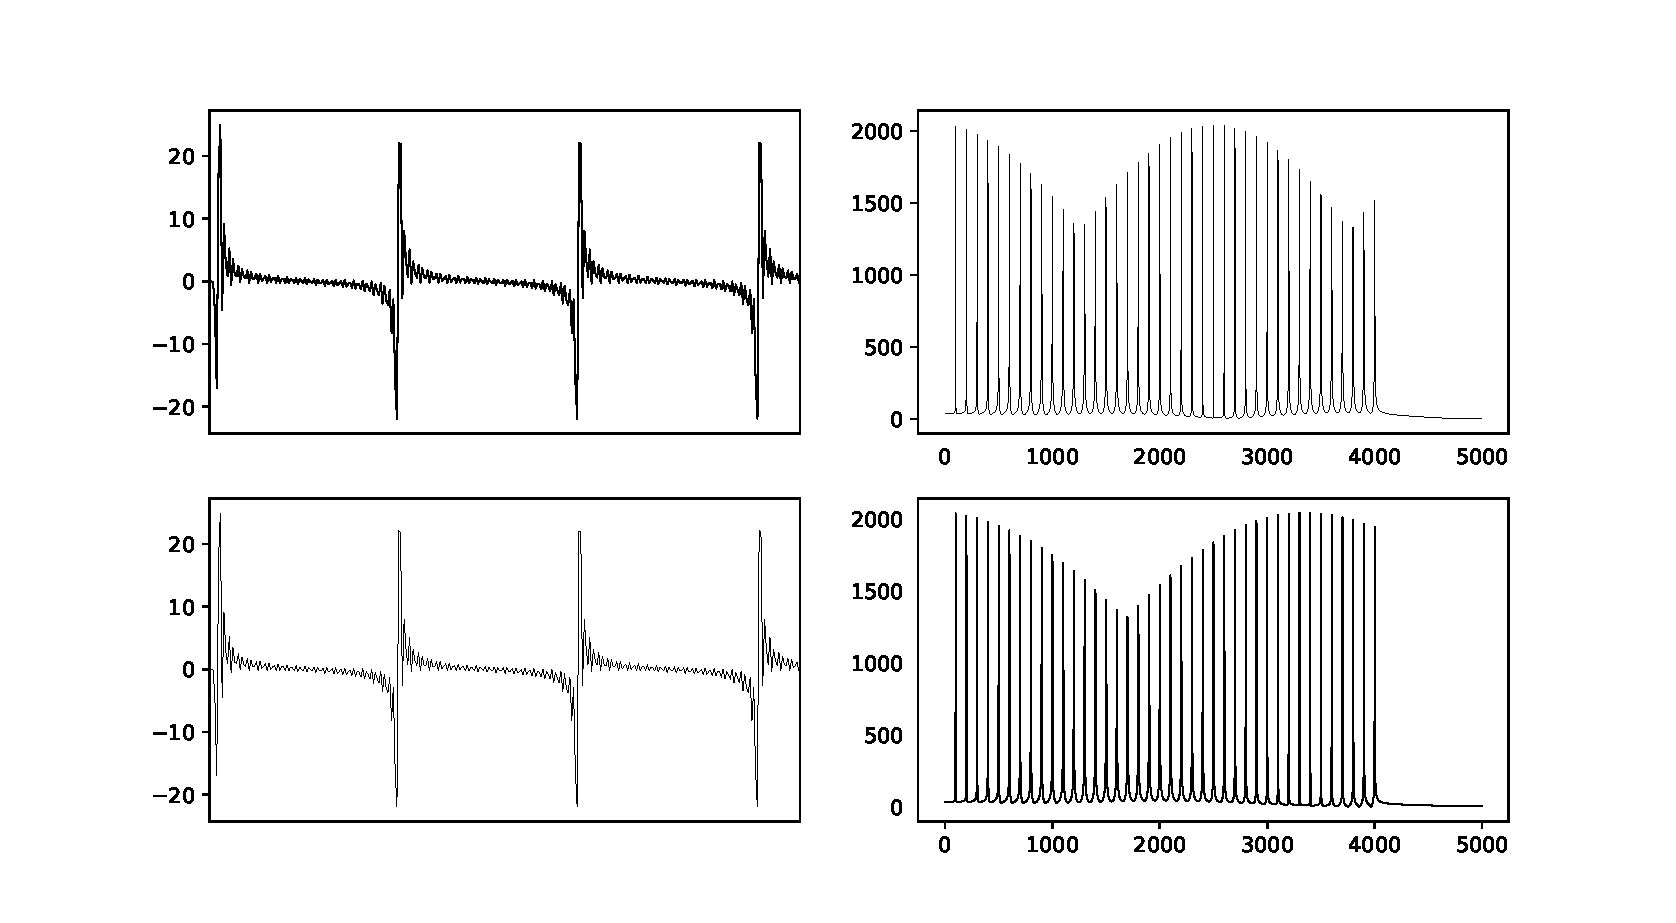
\includegraphics[scale=.55]{Figure_6.pdf}
\caption{(top) is an example of a direct implementation of the Butterworth filter using Scipy lfilter and the Fourier Transform of its output after decimation. (bottom) is the polyphase implementation of the same filter.}
\end{figure} 

Clearly, there is some attenuation loss in the passband that doesn't occur in the direct implementation. The reason for this can be speculated based on the theory from (Schafer and Rabiner, 1973), but was not definitively understood.  We do see, however, that the edge frequencies which fall off in the direct implementation are present in the polyphase implementation.  

The second signal contained the same spacing as the first, but contained 33 components, placing the last component outside the passband.  The result of this is plotted in Figure 3.7.

\begin{figure}[ht]
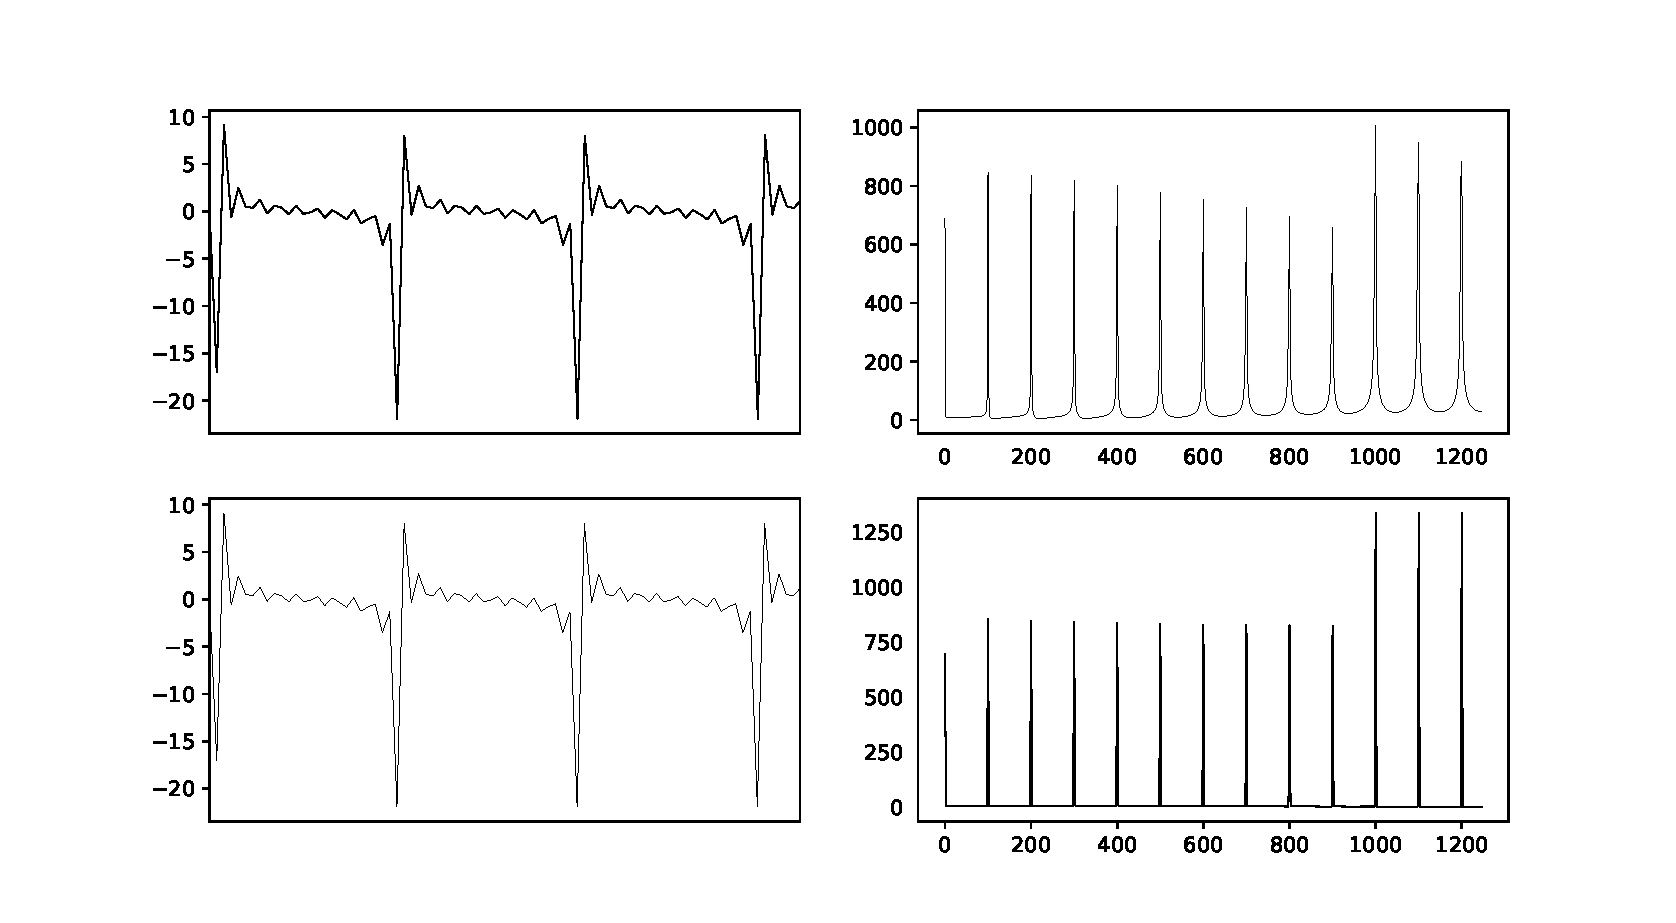
\includegraphics[scale=.55]{Figure_8.pdf}
\caption{(top) is an example of a direct implementation of the Butterworth filter using Scipy lfilter and the Fourier Transform of its output after decimation for the second signal. (bottom) is the polyphase implementation of the same filter for the second signal.}
\end{figure} 

Here we see something rather strange.  While the direct implementation attenuates signals in the stopband as it should, the polyphase implementation does not.  In fact, there is more power in the stopband than there is in the passband.  This error has arisen due to a failure on my part to account for how the filter coefficients and signal would align during the convolution.  For reasons we show later on, it is likely that this is not the only error.

The third signal demonstrates this even more completely, with 60 components, as shown in Figure 3.8.

\begin{figure}[ht]
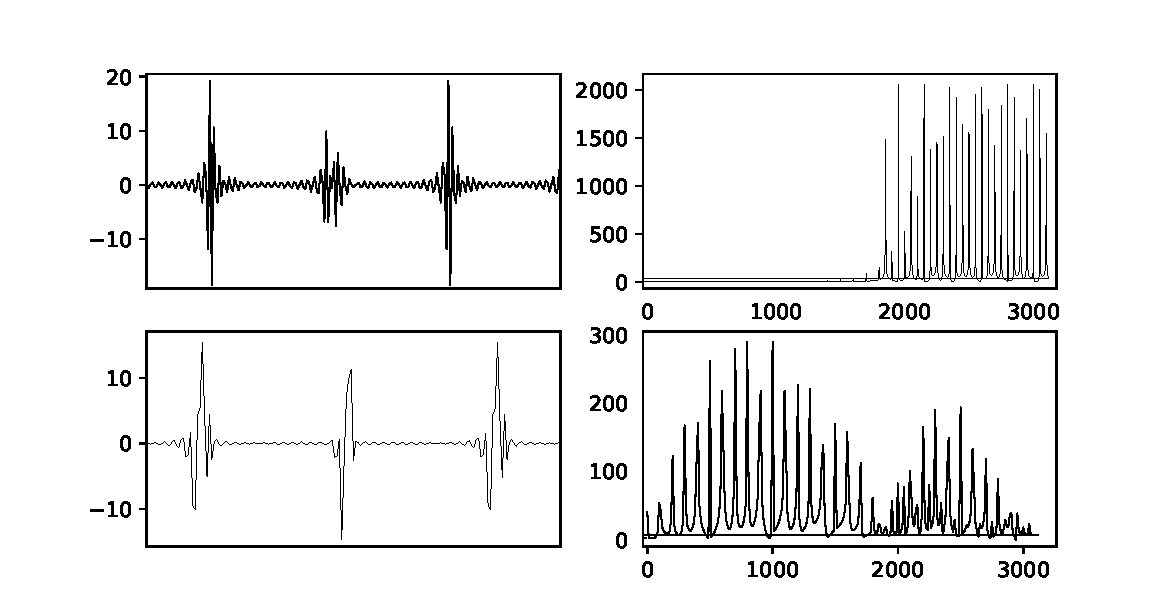
\includegraphics[scale=.55]{Figure_7.pdf}
\caption{(top) is an example of a direct implementation of the Butterworth filter using Scipy lfilter and the Fourier Transform of its output after decimation for the third signal. (bottom) is the polyphase implementation of the same filter for the third signal.}
\end{figure} 

This result is clearly not the anticipated result, since there are frequencies present in the stopband.  There could be several causes.  The first, though unlikely, is how the impulse response of the Butterworth filter is recovered.  This was done by feeding the filter a unit impulse and utilizing the responses.  This may not be the correct method for recovering these coefficients.  The second possibility is that the frequencies in the stopband are actually aliases of the passband frequencies, as they only appear when frequencies higher than the passband frequency appear.  The third is, of course, I have misunderstood a basic aspect of the implementation of the filter bank method, most likely when implementing the time delays for the subconvolutions.  The Schafer and Rabiner paper from 1973 never specifies what a 'good' time delay is, but this implementation assumes a unit time delay, which is what the (Harris 2003) paper shows.  The fourth is that the implementation works fine, and I'm completely misunderstanding the output in these plots.  A more rigorous method would be to look at the frequency responses for each subfilter, as well as for the polyphase method.  Unfortunately, I didn't have time to learn how to accomplish this.  The Scipy library has a method for its built-in filters, but not for a generic set of impulse response coefficients.

In an article on DSP-related (https://www.dsprelated.com/showarticle/191.php), the author mentions a necessary reordering of the coefficients in order to recover the proper alignment.  I did not take this into account, and after investigation of a 3-tap filter using the same process as the example in the section above, it turns out that the recovered coefficients (calculations have been attached) indeed do not match the direct convolution.  Figure 3.9 shows the above, but for a 2-tap implementation with the 60 component signal.  Indeed, the extra power in the stopband is not there. 

\begin{figure}[ht]
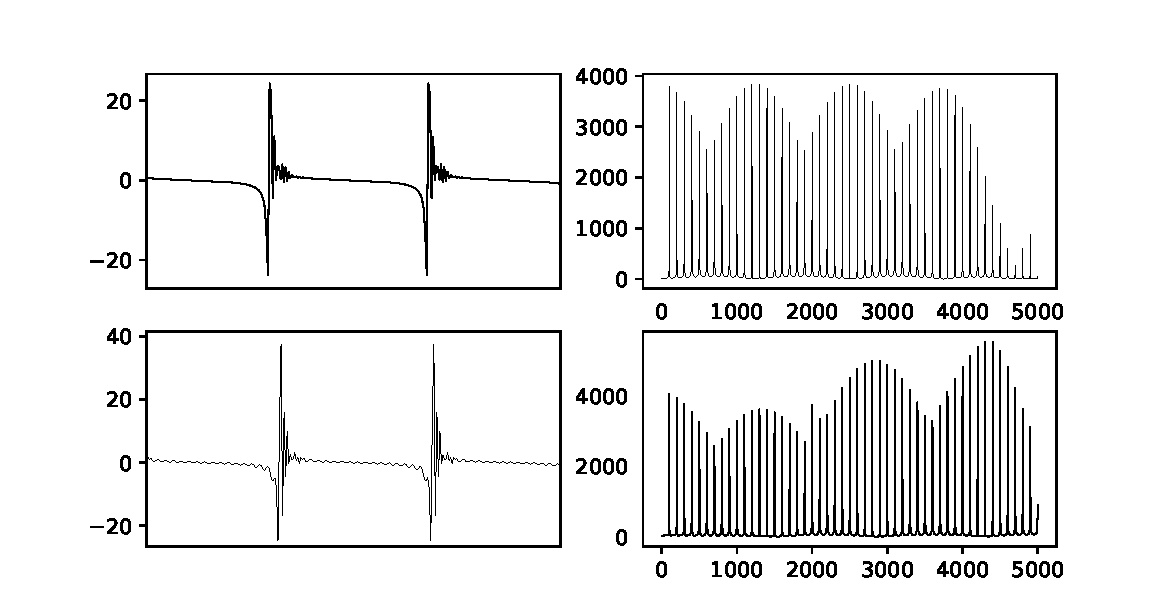
\includegraphics[scale=.55]{Figure_9.pdf}
\caption{This is the examply using a 2-tap implementation instead.}
\end{figure} 

It is likely that there is another issue with the cadence of the signal-coefficient multiplications that I haven't taken into account, since the power should be equal for all frequencies, but there is an odd rolloff.  Unfortunately, I do not have the time to implement a correction, since the error is not completely understood to begin with.  Below is the code utilized in this process.

\#--------------------------------------------------------------------------------------

import scipy.signal as sig

import numpy as np

import matplotlib.pyplot as plt

sin = np.sin

cos = np.cos

pi = np.pi

zeros = np.zeros

rand=np.random.rand

fft = np.fft.fft

def srand():

  return rand()-rand()

def cta(freq):

    return 2*pi*freq
    

'''
Create ideal lowpass filter of Butterworth type with order 48
'''
wNy = cta(fNy)

ubp = cta(10000)/wNy

ubs = cta(11275)/wNy

N, Wn = sig.buttord(ubp, ubs, .1, 50, False)

b, a = sig.butter(N, Wn, 'lowpass', False)

l = len(b)

impulse = np.repeat(0.,l); impulse[0] =1.

x = np.arange(0,l)

resp = sig.lfilter(b,a,impulse)

\# Implementation of a polyphase downsampler

M = 2

N = 4096

signal = FDMSig[:N,0]
 
sbl = int(signal.shape[0]/M)

sigBands = np.zeros([sbl,M])

sigBands[:,0] = signal[::M]

for i in range(1,M):

    sigBands[:,M-i] = signal[i::M]

fbl = int(resp.shape[0]/M)

filtBands = np.zeros([fbl, M])

for i in range(0,M):

    filtBands[:,i] = resp[i::M]
    
subConv = np.zeros([sbl + fbl + (M-1), M])

for i in range(0, M):

    subConv[i:subConv.shape[0]-(M-i), i] = sig.convolve(sigBands[:,i], 
    
            filtBands[:,i], 'full', 'direct')
            
subConv = subConv.transpose()

polyPhaseOut = subConv.sum(axis=0)

'''
Implementation of filtering, then downsampling
'''

filtSig = sig.lfilter(b, a, FDMSig[:,0])

decFiltSig = filtSig[::M]

\#-------------------------------------------------------------------------------------

Here I have omitted the code used to create the signal.

\chapter{Conclusion}

We've given a cursory introduction to the digital signal processing components utilized in the polyphase implementation, discussed briefly the theoretical background for why such an implementation is effective, and attempted a realized implementation, though there was a flaw in how the coefficients were aligned which led to errors in the power spectra.

Well, Dr. Gary, I gave it my best shot, and seemed to have come up short, though I believe I'll be able to correct this and have a functional implementation once I understand the coefficient re-ordering.  I don't plan on giving up, though unfortunately I didn't have enough time to correct the error and turn in this report in time.  

\newpage

\textbf{Bibliography}

F. J. Harris, C. Dick and M. Rice, "Digital receivers and transmitters using polyphase filter banks for wireless communications," in IEEE Transactions on Microwave Theory and Techniques, vol. 51, no. 4, pp. 1395-1412, April 2003.

H. J. Landau, "Sampling, data transmission, and the Nyquist rate," in Proceedings of the IEEE, vol. 55, no. 10, pp. 1701-1706, Oct. 1967.
doi: 10.1109/PROC.1967.5962

J.H., Jr, Hammond,  Purington, E.S.. (1957). A History of Some Foundations of Modern Radio-Electronic Technology. Proceedings of the IRE. 45. 1191 - 1208. 10.1109/JRPROC.1957.278525. 

L. C. Godara, "Introduction to "The heterodyne receiving system, and notes on the recent Arlington-Salem tests"," in Proceedings of the IEEE, vol. 87, no. 11, pp. 1975-1978, Nov. 1999.
doi: 10.1109/JPROC.1999.796359

Pal, Srikanta  J. Lancaster, Michael D. Norrod, Roger. (2012). HTS Bandstop Filter for Radio Astronomy. Microwave and Wireless Components Letters, IEEE. 22. 236-238. 10.1109/LMWC.2012.2193122. 

R. W. Schafer and L. R. Rabiner, "A digital signal processing approach to interpolation," in Proceedings of the IEEE, vol. 61, no. 6, pp. 692-702, June 1973.
doi: 10.1109/PROC.1973.9150


\end{document}
